\documentclass[12pt]{extarticle}
\usepackage[utf8]{inputenc}
\usepackage{cite}
\bibliographystyle{unsrt}
\usepackage{graphicx}


\title{DeepFake Detection with Multi Modal Analysis using Advanced Machine Learning}
\author{Rapolu, Devendra Bupathi\\
\texttt{11639592} 
\and Konda, Shiva Sai\\
\texttt{11596850}
\and Kadasani, Praveen Reddy \\
\texttt{11597360}
\and Bachireddy, Sathvika\\
\texttt{11627310}
}
\date{February 25, 2024}

\begin{document}

\maketitle
\section{Introduction}
Increases in sophisticated technology brought forth by the digital era allow for hitherto unthinkable manipulation of media. The innovation at the center of this transformation is DeepFake, which produces artificially produced pictures and movies that are incredibly lifelike by utilizing advanced machine learning algorithms. Making the distinction between real media and altered stuff is extremely difficult with this technology. DeepFake are becoming more common and harder to identify, which increases the risk of disinformation and its effects on security and privacy in a variety of fields, such as politics, journalism, and social media.

As of right now, we are only examining the literature on DeepFake identification and putting together a test dataset that has both fake and authentic information. Our objective is to create models that can recognize these modifications with accuracy. Our current efforts are focused on assessing the capability of various machine learning algorithms for properly recognizing DeepFake.

For a number of reasons, this project is crucial to our data science education. First of all, it provides a chance to employ intricate data science theories and methods in an actual, useful context. Furthermore, it offers a venue for investigating the harmony between the potential and moral use of machine learning in media. Lastly, it enables us to address a topic that is becoming increasingly important to society: the accuracy of information in the digital era.

We want to get a deeper grasp of important concepts through this research, including feature engineering, the use of sophisticated algorithms like Generative Adversarial Networks (GANs) and Convolutional Neural Networks (CNNs), and the creation of reliable detection models. We also want to learn a great deal about the ethical implications of machine learning, especially as it relates to information sharing and media authenticity.


\section{Statement of the Problem}

The core problem our project addresses is the development of an effective and accurate system for detecting DeepFake content using advanced machine learning techniques. The following questions delineate the scope of our investigation:

\begin{enumerate}
    \item How can various machine learning algorithms, specifically Convolutional Neural Networks (CNNs), Generative Adversarial Networks (GANs), be utilized to detect and differentiate between real and AI-generated DeepFake media?
    \item What are the most effective features and techniques for identifying the subtle nuances that distinguish authentic digital media from DeepFakes?
    \item How can the proposed system be optimized to handle diverse forms of media and manipulation techniques, ensuring robustness and adaptability in detection?
\end{enumerate}

\section{Review of Literature}

The paper \textbf{Salvi, Liu and Mandelli (2023)} introduces an approach in detecting multimodal deepfake videos by combining visual and audio data. Here they used Early Fusion technique and trained on monomodal samples. Their future work will explore the informed fusion methods, modalities based on their application to predict accuracy. \cite{jimaging9060122}

The authors \textbf{Khalid, Tariq and Kim (2021)} introduced a dataset designed to detect both deepfake videos and audios. It has features gender and racial diversity along with age groups. They used methods to create almost true lip-synced videos and audios. Hope these help us to develop more robust deepfake detectors and explore in multimodal deepfake detection. \cite{khalid2021evaluation} \\ \cite{khalid2022fakeavceleb}

This article \textbf{Liu, Tang, Lv and Wang (2018)}  bring us a hybrid multimodal approach which combines video, audio, face movements for reading emotions. These modals were accurate than the previous ones. They faced few issues in AFEW dataset but overcome them by with the dataset STED. \cite{liu2018clips}

From the papers and the datasets that we have gone through, this literature review provides us complete understanding of the existing research, challenges, future directions in the field of deepfake detection. \nocite{Chelehchaleh_Salehi_Farahbakhsh_Crespi_2024}

\section{Objectives of the Study}

\begin{enumerate}
    \item \textbf{To Develop a Comprehensive DeepFake Detection Model:} To construct a sophisticated machine learning model that can accurately identify and differentiate between authentic and DeepFake-generated content. This model aims to incorporate cutting-edge techniques in machine learning for effective detection.

\item \textbf{To Analyze and Optimize Algorithmic Performance:} To explore and determine the most effective combination of algorithms, such as CNNs, GANs, and RNNs, for the specific task of DeepFake detection. This includes an in-depth analysis of each algorithm's strengths and potential synergies when used in conjunction.

\item \textbf{To Enhance Feature Selection and Engineering:} To identify and refine the key features that are most indicative of DeepFake manipulations. This involves a detailed exploration of both the visual and temporal characteristics that distinguish DeepFakes from genuine content.

\item \textbf{To Evaluate Model Robustness Across Diverse Scenarios:} To rigorously test the developed model's performance across various types of content and manipulation techniques, ensuring its effectiveness and reliability in diverse real-world scenarios.
\end{enumerate}

These objectives are designed to guide the research towards developing a highly effective tool for combating the challenge of Deepfake content, thereby contributing significantly to the field of digital forensics and information security.

\section{Research and Design Methodology}
The primary goal of this project is to create a powerful deepfake detection system utilizing GANs and CNNs to separate between the genuine and counterfeit media that is pictures and sound. We have selected these models cautiously as they are vital to do our project, they ought to have a standing and they will be having the option to recognize genuine and fake samples and track down designs in data. By utilizing the preprocessing strategies, we will gather the datasets with both genuine and fake pictures and sounds, ensuring precision and consistency. We utilize this dataset to prepare out information utilizing CNNs and GANs; the CNNs will be utilized to extricate remarkable qualities from the photographs, and the GANs will utilize them to level up their abilities at making sensible looking phony media. Our primary objective in this undertaking is to further develop location considerably further by consolidating the CNN model with the GAN's discriminator part. We will likewise utilize information increase and regularization ways to deal with improved dataset and stay away from overfitting. We will keep on putting a high need on moral issues as we direct our examination to ensure that it consents to moral standards and doesn't advance the ill-advised utilization of deepfake innovation.

\subsection{Machine Learning Approaches}
we explored a number of machine learning methods, such as convolutional neural networks (CNNs) and deep belief networks (DBNs), for identifying DeepFakes. These methods play a crucial role in the analysis and detection of modified content in photos and videos, aiding in the separation of real media from that which has been altered by DeepFake technology. The focus is on how flexible and efficient these techniques are at identifying minute changes that would go unnoticed by the naked eye.

\begin{figure}[htp]
    \centering
    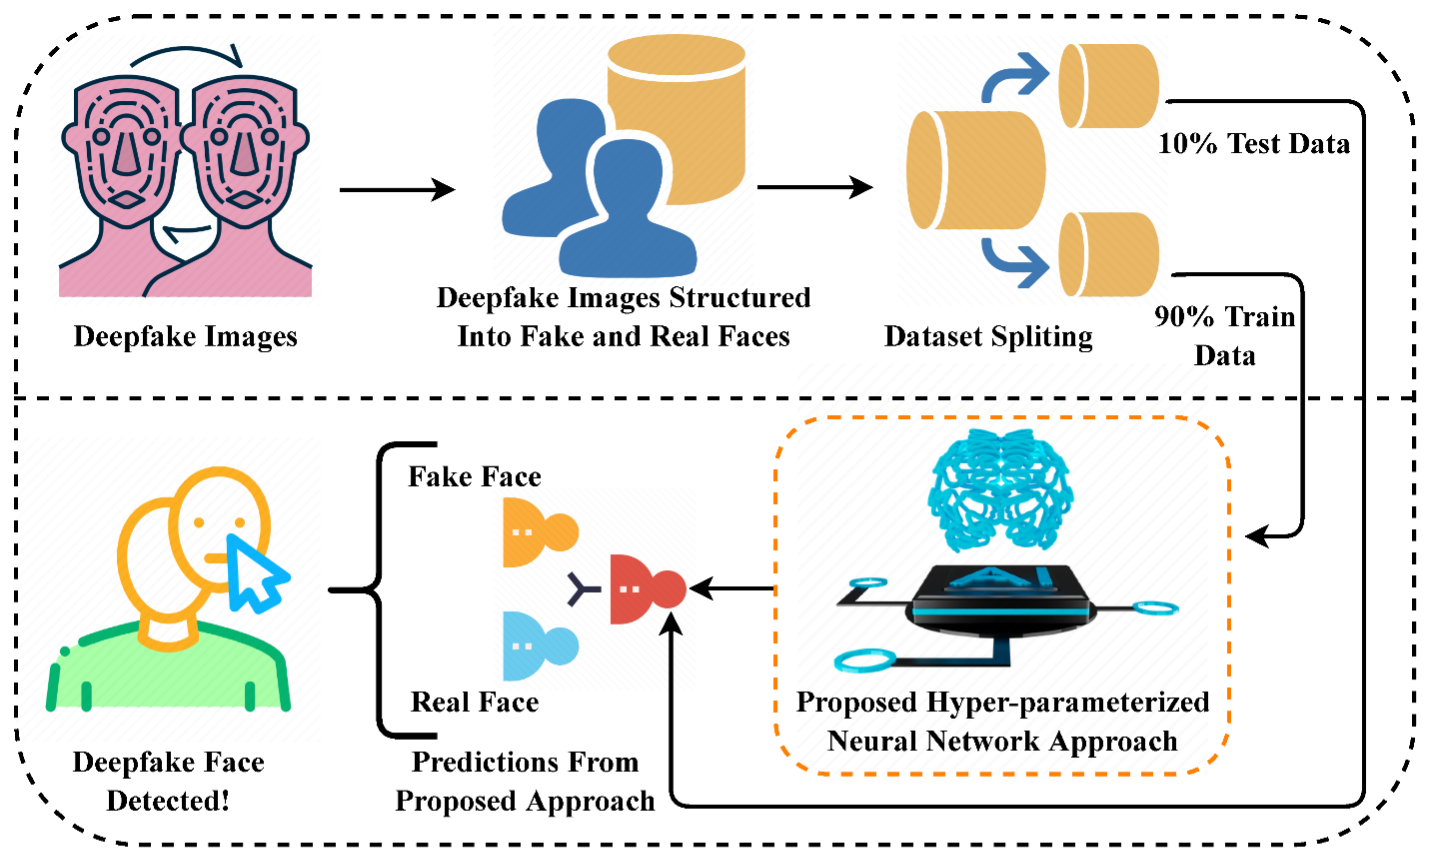
\includegraphics[width=13cm]{Picture1.png}
    \caption{System Architecture}
    \label{fig:galaxy}
\end{figure}

\section{Dataset Description}
The datasets are taken from Kaggle.
There are 2 datasets that are being used in this project.
\begin{enumerate}
    \item \textbf{Audio dataset:}
The raw audio can be found in the "AUDIO" directory. They are arranged within "REAL" and "FAKE" class directories. The audio filenames note which speakers provided the real speech, and which voices they were converted to. For example, "Obama-to-Biden" denotes that Barack Obama's speech has been converted to Joe Biden's voice.\cite{kaggleDeepVoice}

\item \textbf{Image dataset:}
This dataset contains manipulated images and real images. The manipulated images are the faces which are created by various means. The dataset has divided into 3 folders Train,Test,Validation and each of this folder has subfolders fake and real images.\cite{kaggleDeepImages}
\end{enumerate}
\section{Individual Contributions}

\subsection{Devendra Bupathi Rapolu}
Devendra was responsible for leading the project, coordinating the efforts of the team members, and ensuring timely completion of tasks. Devendra also contributed significantly to the writing and compilation of the project proposal.
\subsection{Shiva Sai Konda}
Shiva focused on the data acquisition process, identifying and securing a diverse range of datasets for the project. He was instrumental in preprocessing the data, ensuring it was suitable for analysis and modeling. Shiva also took the lead in feature engineering, identifying key features that could effectively differentiate DeepFakes from authentic content.
\subsection{Praveen Reddy Kadasani}
Praveen contributed significantly to the literature review, providing in-depth insights from the articles and research papers. Their work in documenting the critical processes and steps was essential for the project's methodology.
\subsection{Sathvika Bachireddy}
Sathvika's primary responsibility was conceptualizing the approach to the problem statement. She explored various machine learning models, assessing their applicability and effectiveness for DeepFake detection.


\section{Conclusion}

⁤To summarize, this research creates a machine learning system that can recognize DeepFake audio and images, tackling a significant issue in the digital era. ⁤⁤By taking the advantage of CNNs, GANs, we provide a reliable, multi-modal detection model. ⁤⁤The ethical conversation around AI technology in media is enriched by this model, while promising great accuracy in separating artificial intelligence (AI)-generated media from actual media. ⁤Our effort might have a big influence on information security and digital forensics by improving the identification of DeepFakes, which will help stop the spread of false information. Our research will ultimately help create a digital world that is more genuine and reliable while demonstrating the ethical and responsible applications of AI. 


\bibliographystyle{plain}
\bibliography{M335}

\end{document}
